\section{Introduction}
\label{sec:introdction}
Data exploration has gained lots of attentions over the last few years. The
main challenge is to support users with little prior knowledge, and no clear
objective. Some users need a preliminary impression of the data before engaging
into more structured tasks. Others are browsing in the hope to discover new
insights.  To help them, several authors have proposed systems to ``play'' with
the data~\cite{abouzied2012dataplay, sellam2013meet, liarou2014dbtouch,
dimitriadou2014explore}. These systems offer some textual or graphical
interface, through which explorers can create, visualize and modify selections of
tuples quickly. Thus, users are engaged in a tight trial-and-error loop,
through which they discover their datasets. 

Data exploration systems rely on a crucial assumption: they suppose that if the
users see an interesting set of tuples (e.g., through tables or
visualizations), they will recognize it immediately, and think ``aha, this is
interesting''. This assumption may hold with small datasets, but it collapses
in higher dimensions. If the dataset contains  dozens, or hundreds of columns,
then which variables should the users inspect? Furthermore, which
\emph{combinations} of variables should the user inspect? We cannot assume that
our data explorers know where to look.  Yet, studying each possibility in turn
can turn out to be a slow, tedious process. This beats the purpose of a data
exploration system.
%\begin{framed}
%    \everypar={{\setbox0=\lastbox}\everypar{}}
\textbf{How can we describe an arbitrary set of tuples when the
database contains more than a dozen columns?}
%\end{framed}

The straightforward approach is to use multidimensional visualizations such as
parallel coordinates or small multiples. Unfortunately, these methods tend to
show every possible aspect of the data, thus they do not scale well. For
instance, we would need at least 50 small multiples to visualize a dataset with
only 10 columns. Dimensionality reduction algorithms such as PCA or ICA are
also common, but they ignore the user's selection, and hence may
miss interesting combinations.  Besides, they rescale and rotate the
variables, causing their output to be harder to interpret.

In this paper we introduce our approach, \emph{multi-view subset
characterization}. The key idea is to detect subspaces inside which the user's
selection has an unusual distribution compared to the rest of the database.
These subspaces should be small, interpretable and non-redundant.  We
materialize this idea with Ziggy, a \emph{subset description engine}. For a
given subset of a database, Ziggy automatically generates a description of the
tuples with natural language and visualizations.  Thus, plugged on top of a
database engine, Ziggy can veritably simulate a conversation: the
user issues queries, and Ziggy replies in natural language. Our system can
process 10,000s tuples on dozens of variables within a second, and it can cope with
both numerical and nominal data, including missing values.  Thus, it can
readily replace the output of a data exploration system. To summarize, here are
our contributions: \begin{itemize0}
    \item We introduce and formalize the multi-view subset characterization problem.
    \item We describe Ziggy, a simple, efficient and robust system to describe
        selections of tuples in natural language
    \item We apply our system to real-life situations and benchmark it against
        state-of-the-art algorithms
\end{itemize0}

Our paper is built as follows. In Sections~\ref{sec:genoverview}
and~\ref{sec:problem}, we present our problem. We instantiate this problem in
Section~\ref{sec:instantiation} and describe our algorithms in
Section~\ref{sec:algorithm}. We discuss how to validate our results and report
them in Sections~\ref{sec:validation} and~\ref{sec:reporting}. We describe how
to set parameters in Section~\ref{sec:parameters}. In
Sections~\ref{sec:usecase} and~\ref{sec:experiments}, we apply our solution to
real and synthetic data. Finally, we present related works and conclude in
Sections~\ref{sec:related-works} and \ref{sec:conclusions}.

\section{Overview}
\label{sec:genoverview}
\begin{figure}
  \centering
  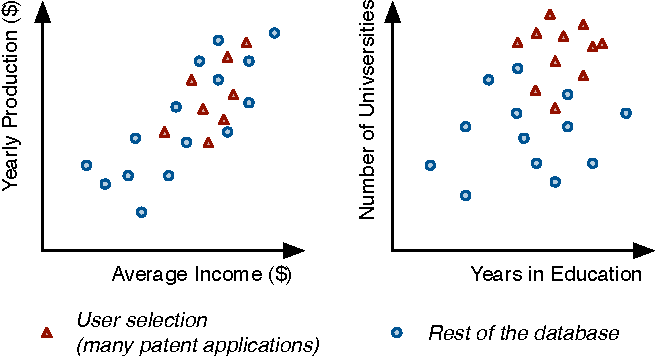
\includegraphics[width=\columnwidth]{Figures/Example}
  \caption{Two examples of subspaces for which the user's selection has an
  unusual distribution.}
  \label{pic:example}
\end{figure}
Let us introduce our problem through an example. A government analyst tries to
understand what demographic, social and economic factors lead to innovation.
More specifically, she is interested in patents: in which parts of the world do
individuals submit patents? What lessons can we learn? To answer this question,
our analyst collects several databases with regional statistics, and loads them
in her favorite business intelligence tool (possibly SQL-based, or
spreadsheet-based). She selects the top 10\% regions for which many patents are
submitted, and ends up with an overwhelming large table, with a few tuples and
hundreds of columns. How can we help her?
 
Our idea is to recommend views, which show how the selection of tuples differ
from the rest of the database. Figure~\ref{pic:example} shows two of these
views. We see that on the columns \texttt{Average Income} and \texttt{Yearly
Production}, the tuples are gathered in top-right corner of the chart. The
effect is even stronger on the second plot, which shows the variables
\texttt{Years in Education} and \texttt{Number of Universities}. Observe that
these views have a purposely low dimensionality. Our aim is not to show
\emph{all} the variables on which the selection has an impact. Instead, we
recommend a few small, non redundant groups, each illustrating one
characteristic of the tuples. We call this approach \emph{multi-view subset
characterization}.

Once we detected the views, we can depict them with visualizations as in
Figure~\ref{pic:example}. The merits of this approach is hardly disputable, in
particular compared to tables. And yet, analyzing charts takes time and
training. Also, not all effects are perceptible, in particular when the views
contain three dimensions or more. Lastly, charts are simply not accessible to
visually impaired users. To address these problems, we propose to exploit a
different communication channel: we generate natural language descriptions of
the views. For instance, we could describe the views pictured in
Figure~\ref{pic:example} as follows:
\begin{quotation}
    On the columns~\texttt{Average Income} and \texttt{Year\-ly Production},
    your selection has a high value and high concentration. The effect is
    similar and stronger on \texttt{Years in Education} and \texttt{Number of
    Universities}.
\end{quotation}
Note that we \emph{describe} the data, but we do not \emph{interpret} it. The
latter problem is much harder, and we claim in no way to have solved it. We
will however dare to issue simple ma\-gni\-tude judgments, such as ``this
effect is particularly strong'', using conservative, transparent hand-written
rules.


\section{General problem statement}
\label{sec:problem}
Let us now formalize the multi-view characterization problem. We represent our
database with a matrix $\rb{D}$, with $M$ columns and $N$ rows.  We model 
each tuples by an iid. random vector  $\rb{x}_n = (x^1_n, \dots, x^M_n)^\top$,
and each column by  $\rb{x}^{m}= (x^m_1, \dots, x^m_N)^\top$.

Let the submatrix $\rb{V}  = [\rb{x}^1, \dots, \rb{x}^V]$ describe a view
(i.e., subspace, or set of columns). We split this view in two:  ${\rb{V}}_t$
contains the tuples in the selection, ${\rb{V}}_{\overline{t}}$ the remainder,
as shown below:
\begin{figure}[h!]
  \centering
  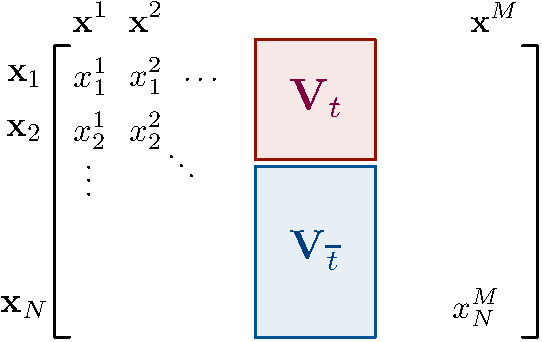
\includegraphics[width=0.5\columnwidth]{Figures/Notations}
%  \caption{Our notations.}
  \label{pic:notations}
\end{figure}


To measure how much $\rb{V}_t$ and ${\rb{V}}_{\overline{t}}$ differ, we compare
the empirical probability distribution of their rows. If these distributions
differ, then the view exhibits some ``peculiarity'' of the data.  Therefore,
$\rb{V}$ is likely to be informative. We measure this difference with a
\textbf{mass dissimilarity measure} $\mf{D}(\rb{V}_t, \rb{V}_{\nott})$.  This
function returns 0 if the tuples come from from the same distribution, it grows
otherwise. The statistics literature contains several candidates, for example
estimators the Kullback-Leibler Divergence~\cite{wasserman2013all}. We will
present our own function in the following section.

We can already propose a first, naive, formulation of our problem:
\begin{problem}
    Consider a distribution dissimilarity function $\mf{D}$ and two integers
    $K$ and $D$. Find the top $K$ distinct views $\rb{V}^i$ with at most $D$
    dimensions which maximize: $ \mf{D}\big( \rb{V}^i_t ;
    \rb{V}^i_{\overline{t}} \big)$ (ignoring column permutations).
\end{problem}

This approach is simple, but it yields redundancy: a small number of good
columns may dominate the results and appear in all $K$ views. In a data
exploration scenario, users may value \emph{diversity}, even if the views are
sub-optimal. To enforce this requirement, we introduce a penalty factor in our
objective function.
\begin{table*}[t!]
    \centering
  \rowcolors{2}{gray!25}{white}
    \begin{tabular}{ccccp{9cm}}
      \hline
    \rowcolor{gray!50}
      Property & Type 1 & Type 2 & Zig-Component & Comments\\
      \hline
      Mean & Contin.  & - &
      $  \mf{z}_m^{\bf{d}}  = (\bar{\bf{d}}_t - \bar{\bf{d}}_{\nott}) / s_{\overline{t}}$ & 
      Known as Glass' $\Delta$~\cite{hedges2014statistical}\\
      Stand. Dev.& Contin.  & - &
      $ \mf{z}_{\sigma}^{\bf{d}}=(s_t-s_{\nott})/s_{\overline{t}}$ & \\
      Frequencies & Discrete & - & 
      $\mf{z}_\chi ^{\bf{d}}= \chi^2$ &
      Pearson's $\chi^2$ goodness-of-fit test~\cite{wasserman2013all}\\
      Dependence & Contin. & Contin. & $\mf{z}_r^{\bf{d}, \bf{d}'}  = r_t - r_{\nott} $ & 
      $r_t$is the correlation coefficient between $\bf{d}_t$ and  $\bf{d}'_t$\newline
      $r_{\nott}$ is the correlation coefficient between $\bf{d}_{\nott}$ and
      $\bf{d}'_{\nott}$~\cite{wasserman2013all}\\
     Dependence  & Discrete & Both & $ \mf{z}_V^{\bf{d}, \bf{d}'} = V_t - V_{\nott} $ &
           $V_t$ is Cram\'er's V coefficient between $\bf{d}_t$ and  $\bf{d}'_t$ \newline
           $V_{\nott}$ is Cram\'er's V coefficient between $\bf{d}_{\nott}$ and
           $\bf{d}'_{\nott}$~\cite{cohen1977statistical} \\ 
      \hline
    \end{tabular}
    \caption{Our choice of Zig-Components for different data types. Each
        component describes a difference, to be evaluated for either each
        column $\bf{d}$ or each couple of columns $\bf{d}, \bf{d}'$ in the
        view. The notations $\bar{\bf{d}}$ and $s$ respectively represent the
        sample mean and sample standard deviation. In the mixed-types case, we
        discretize the continuous column with equi-width binning.}
    \label{tab:dissim}
\end{table*}

Measuring redundancy between column is not straightforward, as this notion is
partially subjective. In our model, we exploit statistical dependency: if two
sets of columns are tightly correlated, then there is a high chance that they
describe the same property of the ``real world''.  Oppositely, if they are
independent, then they probably convey different types of information. From
this observation, we introduce a new version of our problem: we seek views
which maximize the distance statistic, while minimizing inter-view dependency.
We define this problem in a recursive way:
\begin{problem}
    Suppose that we have already detected $i-1$ views ($i > 1$,
    $\rb{V}^{0} = \emptyset$). We obtain $\rb{V}^{1..i-1} = [\rb{V}^1, \ldots,
    \rb{V}^{i-1}]$ by concatenating these views. Let $\mf{S}$ describe a
    statistical dependency measure. Given a positive real $\lambda$, find the
    view $\rb{V}^{i}$ with at most $D$ columns which maximizes:
        \begin{equation}
            \label{prob1}
            \mf{D}\big( \rb{V}^{i}_t  ; \rb{V}^{i}_{\overline{t}} \big) - 
            \lambda \cdot \mf{S} ( \rb{V}^{i} ; \rb{V}^{1..i-1})
        \end{equation}
\end{problem}
Statistics textbooks offer many options to instantiate the dependency measure
$\mf{S}$. Well established examples are multivariate variants of the
correlation coefficient, or the mutual information~\cite{wasserman2013all}.
Here again, we will present our own function in Section~\ref{sec:dependency}.

In Equation~\ref{prob1}, the parameter $\lambda$ controls the trade-off between
mass distance and view diversity: a high value enforces that that the view are
diverse, while a low value expresses our preference for maximizing $\mf{D}(
\rb{V}^{i}_t  ; \rb{V}^{i}_{\overline{t}})$. In practice, this parameter is
not convenient because it has no intuitive scale. For some $L$, an
equivalent way to express our problem is the following:
\begin{equation}
    \label{prob2}
    \begin{aligned}
        & \text{Argmax}_{\rb{V}^{i}} 
            & \mf{D}\big( \rb{V}^{i}_t  ; \rb{V}^{i}_{\overline{t}} \big)\\
        & \text{s.t.} 
        &\mf{S} ( \rb{V}^{i} ; \rb{V}^{1..i-1}) & < L\\ 
    \end{aligned}
\end{equation}
Equation~\ref{prob1} in the Lagrangian of Equation~\ref{prob2}, up to a
negligible additive constant. We prefer this form because the trade-off
parameter $L$ has the same scale as $\mf{S} ( \rb{V}^{i} ; \rb{V}^{1..i-1}) $.
For example, if we instantiate $\mf{S}$ with correlation, then $L$ will simply
describe the maximal acceptable correlation between $\rb{V}^{i}$ and
$\rb{V}^{1..i-1}$.

\section{Instantiation: Meet Ziggy}
\label{sec:instantiation}
We now instantiate the dissimilarity measure $\mf{D}$ and redundancy measure
$\mf{S}$. 

\subsection{Explainable Mass Dissimilarity}
\label{sec:explain}
Let us begin with the dissimilarity~$\mf{D}$. As mentioned previously, we could
borrow any general divergence measure from the statistics literature, such as
the KL-divergence. However, these measurements operate as ``black boxes'': they
describe the intensity of the differences, but they do not explain how the
tuples differ. Our approach is diametrically opposed: we introduce the
\textbf{Zig-Dissimilarity}, a completely \emph{explainable}  mass dissimilarity
measure.

The idea behind the Zig-Dissimilarity is to compute several simple,
interpretable indicators of difference, called \textbf{Zig-Components}, and
aggregate them in a single composite score.  Consider for instance two sets of
tuples $\rb{V}_t$ and $\rb{V}_{\nott}$ with $V$ columns. If these subsets have
the same average for every column, then they probably come from the same
distribution. Oppositely, if the averages are different, then they probably
come from different distributions. From this observation, we can build a simple
dissimilarity measure: for each column $\bf{d}$, we compute the differences
between the means $\bar{\bf{d}}_t - \bar{\bf{d}}_{\nott}$. We obtain
a vector of $V$ Zig-Components. We could add more components by testing other
properties: for example, we could measure the difference between the variance
of each columns.  Finally, we aggregate these components into one composite
indicator: this is is the Zig-Dissimilarity.

\begin{definition}
    A Zig-Component is a function $\mf{z} : \rb{V}\times\rb{V} \to \mathbb{R}$
    which describes one difference between two sets of tuples. If the tuples
    are similar, then $\mf{z}(\rb{V}_t, \rb{V}_{\nott}) = 0$. If not,
    the magnitude of $\mf{z}(\rb{V}_t, \rb{V}_{\nott})$ varies with the strength
    of the difference.
\end{definition}
For the sake of presentation, we  abbreviate $\mf{z}(\rb{V}_t, \rb{V}_{\nott})$
as~$\mf{z}$.

In our implementation, we combined five types of Zig-Com\-po\-nents, summarized
in Table~\ref{tab:dissim}.  Most of them come from the statistics literature,
where they are referred to as \emph{effect sizes}~\cite{cohen1977statistical,
hedges2014statistical}.  We chose these indicators because they have intuitive
interpretations, as well as known asymptotic properties (we will use those
Section~\ref{sec:validation}).  A majority, but not all of them are normalized
and vary between -1 and 1. None of these functions are symmetric, and most of
them change sign according to the direction of the underlying effect.

Observe that Ziggy computes univariate, but also bivariate components: in this
case it compares columns by pairs. Our motivation is to check which
correlations are present in one set and not in the other, or more generally
which correlations are either strengthened or weakened across the datasets. In
the discrete case, we substitute the correlation coefficient by Cram\'er' s V.
This function also measures the associations between two variables, and it
varies similarly between 0 and 1~\cite{cohen1977statistical}. Its value is
$\sqrt{X/(N(\min(l,c) - 1))}$, where $X$ is Pearson's $\chi^2$ statistic and
$(l,c)$ are the dimensions of the contingency table of $\bf{d}_t$ and
$\bf{d}_{\nott}$.

Once we computed the Zig-Components $\mf{z}_1, \ldots, \mf{z}_Z$, we obtain the
Zig-Dissimilarity as follows. First, we compute the absolute values
$|\mf{z}_1|, \ldots, |\mf{z}_Z|$ for each component. We then normalize the
values across components of same type. We obtain a set of intermediary scores
$z_1, \ldots, z_Z$. We aggregate these scores with a weighted sum.
These operations give us one scalar indicator, which summarizes the magnitude
of all the differences.

\begin{definition}
    Let $z_1, \ldots, z_Z$ represent a set of normalized absolute values of
    zig-components, and $w_1, \ldots, w_Z$ a set of user-defined weights.  We
    define the Zig-Dissimilarity as follows: 
    \begin{equation}
        \mf{D}_{Zig}(\rb{V}_t, \rb{V}_{\nott}) 
        \equiv \sum_{k \in [1, Z]} w_k \cdot z_k(\rb{V_t}, \rb{V}_{\nott})
    \end{equation}
\end{definition}
We insist that the Zig-Components must be normalized before the aggregation.
In the general case, we cannot assume that the scores are commensurate.

The aim of the weights $w_k$ is to balance the effects across column types. For
instance, we measure two components for the numerical columns, and only one for
categorical data.  Thus, we set $w_k = 1/2$ for the former and $w_k = 1$
for the latter.  These parameters also let users express their preferences: for
example, a novice user may value one-dimension Zig-Components over those based
on correlation.

Table~\ref{tab:dissim} shows that we measure differences in spaces of one and
two dimensions only.  In principle, we could test spaces with more dimensions.
We chose not to do so, for two practical reasons. First, we suppose that
relationships in three dimensions or more are harder to convey and understand
in natural language.  Second, the number of relationships to be inspected grows
exponentially with the dimensionality of the test. This property harms Ziggy's
runtime, and it leads to much longer outputs. We will show in
Section~\ref{sec:experiments} that this Naive Bayes-like design choice has little
practical effect on the accuracy of our model.


\subsection{Dependency Measure}
\label{sec:dependency}
\begin{figure}
  \centering
  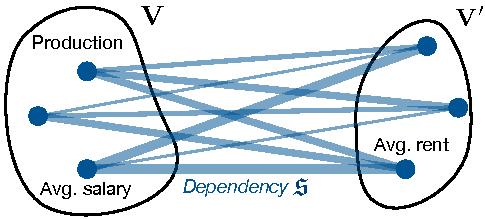
\includegraphics[width=0.6\columnwidth]{Figures/Redundancy}
  \caption{Illustration of Ziggy's redundancy measure. Vertices represent
  column, edges represent pairwise dependency.}
  \label{pic:redundanct}
\end{figure}
We now present two instantiations for the measure of redundancy,
$\mf{S}_{hard}$ and $\mf{S}_{soft}$.  Both measures are a variant of the same
principle, and we will refer to them collectively as the Zig-Dissimilarity
$\mf{S}_{Zig}$. Here again, the main idea is to aggregate several simple
interpretable indicators, such as those that users can find in statistics
textbooks.

Let  $\rb{V}$ and $\rb{V}'$ represent two views. We compute the Zig-Dependency
in two steps. First, we compute the pairwise dependency $\mf{s}(\rb{d},
\rb{d}')$ between every column $\rb{d}$ of  $\rb{V}$ and every column $\rb{d}'$
of $\rb{V}'$, as shown in Figure~\ref{pic:redundanct}. The measure $\mf{s}$ is
a convenience function, which allows us to combine different types of
variables:
\begin{equation}
    \mf{s}(\rb{d}, \rb{d}')= \begin{cases}
        r(\rb{d}, \rb{d}')\ \text{if $\bf{d}, \bf{d}'$ are continuous (correlation)}\\
        V(\rb{d}, \rb{d}')\ \text{otherwise (Cram\'er's V)}
         \end{cases}
\end{equation}
During the second step, we aggregate these dependencies. The function
$\mf{S}_{hard}$ utilizes the maximum, while $\mf{S}_{soft}$ uses the mean:
\begin{gather}
    \mf{S}_{hard}(\rb{V}, \rb{V}') = \max_{d \in \rb{V}, d' \in \rb{V}'} |\mf{s}(d, d')|\\
    \mf{S}_{soft}(\rb{V}, \rb{V}') = 
    \frac{\sum_{d \in \rb{V}, d' \in \rb{V}'} |\mf{s}(d, d')|}
    {V \cdot V'}
\end{gather}
Both functions $\mf{S}_{soft}$ and $\mf{S}_{hard}$ vary between 0 and 1, 0
indicating no dependency. The crucial difference lies in how they treat
overlap. If one column is present in both $\rb{D}$ and $\rb{D}'$, then
$\mf{S}_{hard}$ is at its maximal value 1. This is not necessarily the case for
$\mf{S}_{soft}$. Thus $\mf{S}_{hard}$ leads to less redundancy, while
$\mf{S}_{soft}$ is more flexible. We will demonstrate these effect in our
Experiments section.

Finally, observe that our choice for $\mf{S}$ is computationally efficient: we
get the pairwise correlations for free, because we need to compute them anyway
to obtain the Zig-Dis\-si\-mi\-la\-ri\-ties. 


\section{Algorithms To Detect Views}
\label{sec:algorithm}

We introduced a mass dissimilarity measure $\mf{D}_{Zig}$ and a view dependency
measure $\mf{S}_{Zig}$ (with its two variants). We now discuss how to maximize
the former while constraining the latter.

\subsection{Overview}
\label{sec:overview}

\begin{figure}
  \centering
  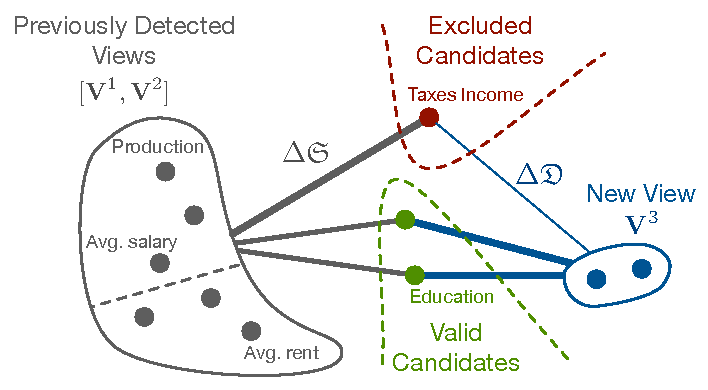
\includegraphics[width=0.8\columnwidth]{Figures/Greedy}
  \caption{Illustration of Ziggy's greedy view composition algorithm, with
  $i=3$ and $D=3$. The grey edges represent the
  amount of redundancy added by each candidate. The blue edges represent the
  amount of dissimilarity added by each candidate.}
  \label{pic:greedy}
\end{figure}
Ziggy operates in two steps. First, it computes the individual Zig-Components
for all the columns in the database. Then, it composes the views in a  greedy
manner. For each view, Ziggy detects which columns are eligible (i.e., do not
violate the redundancy constraint) and it adds those associated with the highest
Zig-Components.

The first step is straightforwards, but it is also by far the most time
consuming. We discuss in Section~\ref{sec:optimization} how to optimize it.
During the second step Ziggy creates the views by adding columns one by one.
Figure~\ref{pic:greedy} illustrates this approach. Suppose that Ziggy has
already obtained two views, $\rb{V}^1$ and $\rb{V}^2$, and it is currently
building a third one, $\rb{V}^3$. For each column in $\rb{V} \setminus \rb{V}^3
$, our algorithm computes two scores: the gain of dissimilarity $\Delta\mf{D}$
induced by adding the candidate to $\rb{V}^3$, and the gain of
redundancy~$\Delta\mf{S}$ induced by the same. Ziggy excludes the columns which
exceed the redundancy capacity, e.g., those for which $\mf{S}([\rb{V}^1,
\rb{V}^2], \rb{V}^3) + \Delta\mf{S} > L$, where $L$ is the dependency limit
introduced in Equation~\ref{prob2}. It then detects the best node among those
that remain (that is, that for which $\Delta\mf{D}$ is maximal) and adds it to
the view. It repeats the process until either the maximal number of columns is
met, or there are no more eligible columns.

In practice, care must be taken when computing $\Delta\mf{D}$, because one
column is often involved in several Zig-Components. Suppose for instance that we
are building a view $\rb{V}^{i}$, and we wish to compute $\Delta\mf{D}$ for
a given candidate $\bf{d}$.  In our
implementation, if $\bf{d}$ contains numeric values, then it will be associated with
at least two components: the difference between the means $\mf{z}_\mu$, and the
difference between the standard deviations $\mf{z}_\sigma$.  Additionally, we must
account for the difference between dependencies, for all the columns
already included in $\rb{V}^{i}$. Thus, if $z$ describes the normalized absolute
value of a Zig-Component $\mf{z}$, and if $\rb{V}^{i}_{num}$ and
$\rb{V}^{i}_{cat}$ respectively represent the numerical and categorical
variables of $\rb{V}^{i}$ the final score is:
%\begin{equation}
    \begin{multline}
\Delta\mf{D} = 
z_\mu^{\bf{d}}+ z_\sigma^{\bf{d}} +
\sum_{\rb{d}' \in \rb{V}^i_{num}} z_r^{\rb{d}, \rb{d}'}
+ \sum_{d' \in \rb{V}^i_{cat}} z_V^{\rb{d}, \rb{d}'}
\end{multline}
%\end{equation}
The last two terms of the equation depends on the current state of $ \rb{V}^i$.
Therefore we must update $\Delta\mf{D}$ after each step.


The choice of dependency measure $\mf{S}_{hard}$ or  $\mf{S}_{soft}$ influences
the correctness of our algorithm. With $\mf{S}_{hard}$, Ziggy will return an
optimal solution. This is not the case with $\mf{S}_{hard}$.  {\color{red} I
    will write a little proof here. - Basically, we are dealing with a variant
of the knapsack problem.}

Finally, if we use the redundancy measure $\mf{S}_{hard}$, then we can avoid
computing $ \Delta\mf{S}$ altogether: Ziggy can discard the redundant
candidates before it starts building the view.  Consider a candidate column
$d$, and let $\rb{V}^{1..i-1}$ describe the union of all previously encountered
views. If $\mf{S}_{hard} (\rb{V}^{1..i-1}, d) > L$, then the column is not
exploitable: adding it to the current view $\rb{V}^{i}$ will breach the
threshold, regardless of $\rb{V}^{i}$'s current state.  Conversely, if we have
$\mf{S}_{hard}(\rb{V}^{1..i-1}, d) < L$, then candidate is ``safe'', it will
never cause the dependency threshold to be breached.  Thus Ziggy, builds the
view in two separate steps: first it eliminates the redundant columns (i.e.,
those for which $\mf{S}_{hard} (\rb{V}^{1..i-1}, d) > L$), then it selects the
top $D$ candidates.  Unfortunately, this property does not hold for
$\mf{S}_{soft}$: we must recompute the value $\Delta\mf{S}$ for each column
after each update of~$\rb{V}^{i}$.

\begin{table*}[t!]
    \centering
  \rowcolors{2}{gray!25}{white}
    \begin{tabular}{c c c c p{8cm}}
    \rowcolor{gray!50}
      \hline
      Property & Type 1 & Type 2 & Test Statistic & Comment\\
      \hline
      Mean & Contin.  & - & $(\bar{\bf{d}}_t - \bar{\bf{d}}_{\nott})/s_{\bar{\bf{d}}_t - \bar{\bf{d}}_{\nott}}$ &
        Wald test~\cite{wasserman2013all}  \\
        Stand. Dev.& Contin.  & - & $s_t / s_{\nott}$ &
        F-test~\cite{cohen1977statistical} \\
        Frequencies & Discrete & - & $\chi^2$ & Pearson's $\chi^2$
        test~\cite{wasserman2013all}\\
      Dependence  & Contin. & Contin & $(Z^{\bf{d}, \bf{d}'}_t - 
      Z^{\bf{d}, \bf{d}'}_{\nott})/s_{Z_t - Z_{\nott}}$ & $Z^{\bf{d}, \bf{d}'}$ is Fisher
      Z-transformation of the correlation coefficient $r$ between $\bf{d}$ and
      $\bf{d}'$~\cite{fisher1915frequency}  \\
      Dependence  & Contin. & Both &  $(V^{\bf{d}, \bf{d}'}_t -
      V^{\bf{d}, \bf{d}'}_t)/s_{V_t-V_{\nott}}$ & $V$ is
      Cram\'er's V. We approximate its distribution with Fisher's
      Normal approximation of $\sqrt{\chi^2}$~\cite{patel1996handbook}.\\ 
      \hline
    \end{tabular}
\caption{Our choice of tests, corresponding to each Zig-Component. We use the
same notations as in Table~\ref{tab:dissim}.}
    \label{tab:tests}
\end{table*}
\begin{figure}[t!]
    \centering
    \begin{subfigure}[b]{\columnwidth}
    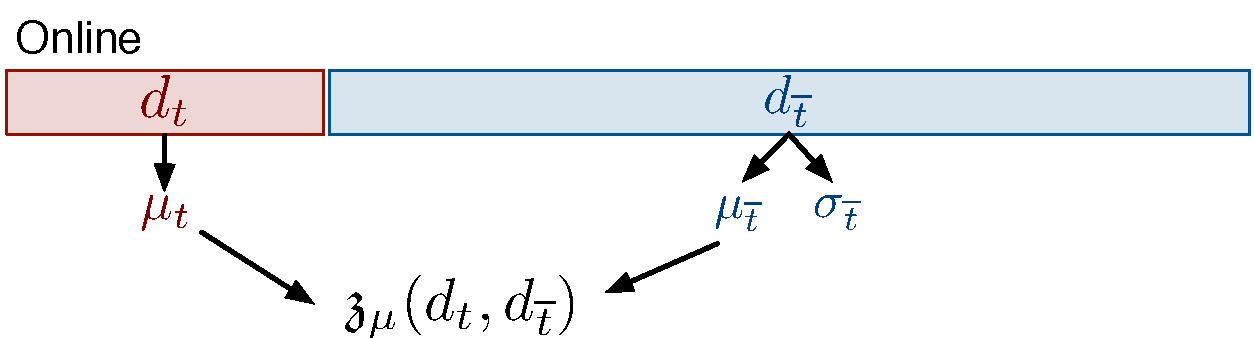
\includegraphics[width=\textwidth]{Figures/Staging}
    \caption{Computing $\mf{z}_\mu$ without staging.}
    \label{pic:withoutstag}
    \end{subfigure}

    \begin{subfigure}[b]{\columnwidth}
        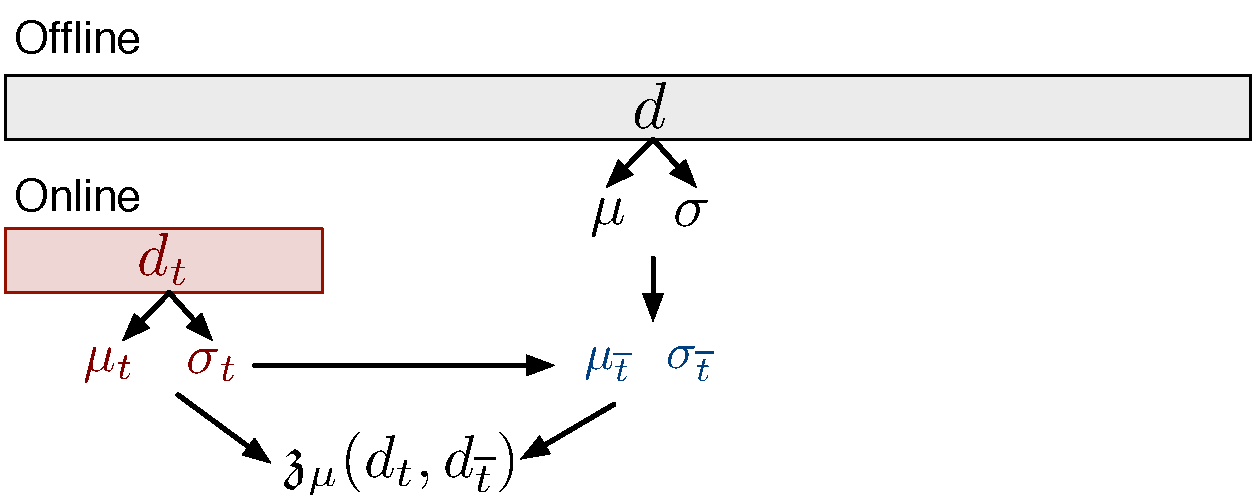
\includegraphics[width=\textwidth]{Figures/Staging2}
    \caption{Computing  $\mf{z}_\mu$  with staging.}
    \label{pic:withstag}
    \end{subfigure}
    \caption{Our staging strategy.}
\end{figure}


\subsection{Staging Computations}
\label{sec:optimization}

We now discuss how to compute the Zig-Components for each column of the
database. This task is critical: in the best case, it requires a full scan of
the database. In the worst case it runs in $\mathcal{O}(N \cdot M^2)$, because
we need to compute to and compare every possible pair of correlations in
$\rb{V}_t$ and $\rb{V}_{\nott}$ for the scores $\mf{z}_r$ and $\mf{z}_V$.

Our idea is to prepare some computations offline, before the user starts
submitting queries.  Let us focus on the Zig-Component $\mf{z}_\mu$, which
reports the difference $(\bar{\bf{d}}_t - \bar{\bf{d}}_{\nott})/{s_{\nott}}$,
for a given column $\bf{d}$ of the database.  Figure~\ref{pic:withoutstag}
presents the naive method to compute this component.  As soon as our user
submits a selection, we compute the average $\bar{\bf{d}}_t$ for those tuples,
the values $\bar{\bf{d}}_{\nott}$ and $s_{\nott}$ for the rest of the database,
and we apply the formula $(\bar{\bf{d}}_t - \bar{\bf{d}}_{\nott})/{s_{\nott}}$
directly. Thus, we read the whole column.

Figure~\ref{pic:withstag} illustrates our staging strategy. Offline, we compute
the mean $\bar{\bf{d}}$ and the standard deviation $s$ for the whole
column~$\bf{d}$. Online, when the user submits a selection, we compute
$\bar{\bf{d}}_t$ and $s_t$
only - thus, we read the selection and ignore the rest of the database. We then
reconstitute $\bar{\bf{d}}_{\nott}$ and $s_{\nott}^2$, as follows:
\begin{gather}
    N_{\nott} = N - N_t\\
    \bar{\bf{d}}_{\nott}= \frac{ N \cdot \bar{\bf{d}} -  N_t \cdot \bar{\bf{d}}_t } { N - N_t } \\
    s_{\nott}^2 = s^2 - s_t^2 -
    (\bar{\bf{d}}_t - \bar{\bf{d}}_{\nott})^2 \cdot \frac{N_t \cdot N_{\nott}}{N^2}
\end{gather}
We now have all the elements to compute the Zig-Component. To obtain these
equations, we used formulas designed to compute the mean and variance
incrementally~\cite{pebay2008formulas}, and we reversed them - in fact we
compute $\bar{\bf{d}}_{\nott}$ and $s_{\nott}$ in a ``decremental'' fashion.

In effect, this method does not reduce the complexity of the algorithm, but it
greatly reduces the amount of tuples to read. The smaller the user's selection
is, the greater is the performance gain. Fortunately, we managed to extend it
for all the Zig-Components presented in Table~\ref{tab:dissim}.  We can derive
similar computations to update correlation
coefficients~\cite{pebay2008formulas}. To cope with categorical data, our
approach is slightly different. Offline, we compute a histogram for $\bf{d}$.
Online we compute another histogram for $\bf{d}_t$. From those, we can infer
the distribution of $\bf{d}_{\nott}$'s values, and compute $\mf{z}_\chi$ and
$\mf{z}_V$.

\section{Model Validation}
\label{sec:validation}

We now focus on the following problem: for a given view $\rb{D^i}$, how
\emph{significant} is the Zig-Dissimilarity $D = \mf{D}( \rb{V}^i_t  ;
\rb{V}^i_{\overline{t}})$? A high value may indicate that $\rb{V}^i_t$ and
$\rb{V}^i_{\overline{t}}$ come from two different distributions.  But it could
also be caused by chance. How confident are we of this result? Answering this
question has two practical uses. First, a confidence score can help us decide
when to stop generating views. Second, it helps users interpret Ziggy's results.

The statistics literature proposes a completely ge\-ne\-ric way to solve
this problem: permutation testing. This methods works with the Zig-Dependency,
but it can also handle other divergence measures. The main idea is to
repeatedly shuffle the rows of $D^i$, without modifying $\rb{t}$. Thus, the
tuples are randomly affected to $\rb{V}^i_t$ and $\rb{V}^i_{\overline{t}}$. We
then observe how the dissimilarity varies: if the permutations have no
effect on $D$, then there is high chance that the dissimilarity was caused by
chance.  Oppositely, if $D$ is very sensitive,
then we have a high confidence in our result. We refer the interested
reader to Wasserman~\cite{wasserman2013all} for more details.

Permutation testing offers plenty of advantages, but shuffling the rows is
computationally heavy. In our implementation, we used an alternative approach.
The main idea is to use the composite nature of the Zig-Dissimilarity, and test
each Zig-Component individually. We then aggregate these scores in a synthetic
confidence indicator. Therefore we do not test the Zig-Dissimilarity directly -
instead we focus on its underlying effects.  This method is much lighter
because we can use known asymptotic results, or at least approximations
thereof. For instance, we know that under certain assumptions, we can test the
difference between the means with a Wald test~\cite{wasserman2013all}, which
only requires an extra $\mathcal{O}(1)$ computation.  Similarly, we can use a
F-test for the ratio of the variances, or a $\chi^2$ test for the differences
in categorical distributions.  Table~\ref{tab:tests} summarizes our choices. 
To aggregate the tests, we report the minimum observed p-value. We must note
that this approach is very conservative. More flexible alternatives include
the Bonferroni corrections, or the Benjamini-Hochberg
method~\cite{wasserman2013all}.

\section{Report Generation}
\label{sec:reporting}
\begin{figure}[t!]
  \centering
  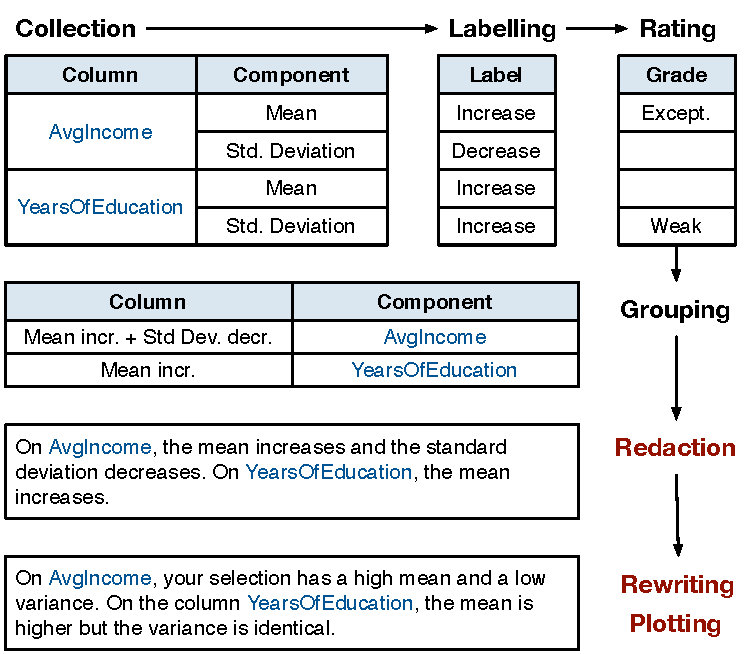
\includegraphics[width=\columnwidth]{Figures/ReportGeneration}
  \caption{Ziggy's report generation pipeline.}
  \label{pic:reportpipeline}
\end{figure}
\begin{table}[t!]
    \centering
    \begin{tabular}{| p{4.2cm} | c | c |}
      \hline
      Description & Exceptional? & Weak?\\
      \hline
      $\mf{z_\mu} \geq 0$ and $\mu_{\nott} \geq 0$: ``increase'' &
          \multirow{4}{*}{$z_\mu$ in top 5\%} & 
            \multirow{2}{*}{$|\mf{z_\mu}| < 0.2$}\\
      $\mf{z_\mu} \geq 0$ and $\mu_{\nott} < 0$: ``decrease'' &
      &\\
      $\mf{z_\mu} < 0$ and $\mu_{\nott} \geq0$: ``increase'' &
       &\multirow{2}{*}{$p_\mu < 0.01$}\\
      $\mf{z_\mu} < 0$ and $\mu_{\nott} < 0$: ``decrease'' &
      &\\
      \hline
    \end{tabular}
    \caption{Example of handwritten rules for the difference of means
    $\mf{z_\mu}$. The variable $p_\mu$ describes the confidence (p-value), as
described in Section~\ref{sec:validation}.} 
\label{tab:handwritten}
\end{table}

We explained how our system detects views. We now detail Ziggy's report generation
pipeline, through which it justifies its choices. 

Ziggy describes its views one by one. For each view, it generates a report,
comprising a few sentences and several charts. The aim of the text is to give a
general presentation of how the tuples differ from the rest of the data. The
charts let users inspect the details.  Figure~\ref{pic:reportpipeline}
illustrates how Ziggy proceeds. First, it gathers all the Zig-Components
associated with each columns of the database. It then generates a short
description for each component, using hand-written rules such as those
presented in the first column of Table~\ref{tab:handwritten}. It also evaluates
each component, with a scale of three grades: ``weak'', ``neutral'', and
``exceptional''. These grades are based on the confidence scores discussed in
Section~\ref{sec:validation}, the absolute value of the effects, and their
relative values compared to other effects of the same type. We illustrate them 
with the two last columns of Table~\ref{tab:handwritten}. These grades
influence how Ziggy presents the statistics: the weak values are treated
separately, and the strong values are emphasized. To set the thresholds, we
took inspiration from classic statistics textbooks~\cite{cohen1977statistical},
and chose conservative options.  Nevertheless, these quantities are inherently
arbitrary. It is therefore important to communicate them to the end
users, and motivate each decision with its corresponding rule.

Once Ziggy has collected, labeled and rated the Zig-Comp\-onents, it  groups
the columns which have the same ``profile'', that is, the same variations on the
same components. It then generates one sentence for each group, such that
each sentence has the same structure: \texttt{on [column\_names], the
[zig-component] [label]}. If several components are involved, as in
Figure~\ref{pic:reportpipeline}, the Ziggy enumerates all the pairs
\texttt{[zig-component] [label]}. At this point, the text produced is
understandable, but it is also highly redundant and grammatically incorrect. During the
rewriting phase, Ziggy remedies this situation a set of handwritten rules. Such
rules include inserting connectors (e.g., ``Additionally'', ``Finally''), using
random synonyms (e.g., ``the tuples'', ``the selection'', ``your data'') or
replacing wider chunks of text (e.g., ``has a lower variance'' by ``spreads
more widely'').

By default, Ziggy only produces visualizations for the variables associated
with exceptional components. It plots the remainder on demand. To determine
which type of visualization to use, it checks the type of the columns, and
applies usual techniques: it uses density plots and histograms for one
dimension data, and scatterplots and heat maps for two-dimension data.

\section{Setting Parameters}
\label{sec:parameters}

Ziggy's model relies on three parameters: the total number of views $K$ to
generate, the width of the views $D$, and the dependency threshold $L$. 

\textbf{Number of Views K.} When should we stop producing views? We propose to
generate as many views as possible, and delegate the final decision to the
users - after all, we have little idea about what they seeking. In practice, we
can do so lazily: we start with a small selection of views (e.g., as many as
the display can contain), and we generate the remainder on demand, for instance
with a ``show me more'' button.  In our experience, the number of views stays
manageable because the algorithm is blocked by the redundancy constraint: after
a certain number of views, Ziggy finds no more columns to exploit. If the views
have a low confidence (as detailed in Section~\ref{sec:validation}), then Ziggy
issues a warning.

\textbf{Size of the Views D.} In our implementation, we set this parameter in an adaptive
fashion, using a method presented by Zhu and Ghodsi~\cite{zhu2006automatic}.
The main idea is the following. When building a view, we keep track of the
gains $\Delta\mf{D}_d$ induced by each column $d$.  We then detect change
points in the sequence (e.g., ``jumps'' or ``elbows'').  If we observe such a
behavior, we truncate the current view and start a new one.  The advantage of
this method is that $D$ can adapt to each subspace. However, it is
only a heuristic. Fortunately, inaccuracies have little consequence in
practice: if the dependency constraint is weak, then the excluded columns are
simply pushed to the next view.

\textbf{Dependency threshold L.} Admittedly, there is no optimal way to set
this parameter: it depends entirely on the user and the exploration context. By
default, we use $\mf{S}_{hard}$, and we limit to $L=0.99$. This setting
enforces that the views are non-overlapping, but it adds no other constraint -
we see this as a safe option.

\textbf{Zig-Components.} Previously, we proposed several Zig-Components, in
order to capture a wide range of effects. In practice, nothing forces to use
them all. For instance, a user interested in quick and concise results may
prefer to ignore the bivariate components.


\section{Use Case}
\label{sec:usecase}

\begin{table}[!t]
    \centering
    \small
    \begin{tabular}{p{4cm} c c c} 
        \hline
        \multirow{3}{*}{Columns}  & Except. & Weak  & \multirow{3}{*}{Score}\\
                                  & Comp.   & Comp.& \\
                                  & (\%)    & (\%)& \\
        \hline
        Patent\_applications\_per\_million & \multirow{3}{*}{83.3}
        &\multirow{3}{*}{0} & \multirow{3}{*}{25.4} \\
        PCT\_patent\_applications&&&\\
        Personal\_earnings &&&\\
        \hline
        Dwellings\_no\_basic\_facilities&
        \multirow{4}{*}{64.2} &\multirow{4}{*}{7.1} & \multirow{4}{*}{18.9} \\
        Educational\_attainment&&&\\
        Emp.\_work\_very\_long\_hours&&&\\
        Life\_expectancy&&&\\
        \hline
        Average\_hours\_worked&
        \multirow{4}{*}{50} &\multirow{4}{*}{42.2} & \multirow{4}{*}{12.4} \\
        Population\_growth\_rates&&&\\ 
        Working\_age\_population&&&\\
        Pop\_under\_the\_age\_of\_15&&&\\
        \hline
        Assault\_rate, Homicide\_rate &
        \multirow{2}{*}{77.7} &\multirow{2}{*}{11.1} & \multirow{2}{*}{12.1} \\
        Current\_\-account\_balance&&&\\
        \hline
        Export\_Pharmaceutical&
        \multirow{4}{*}{57.1} &\multirow{4}{*}{57.1} & \multirow{4}{*}{11.4} \\
        Incidence\_part\_time\_emp&&&\\ 
        Long\_term\_unemp&&&\\ 
        Production\_crude\_oil&&&\\ 
        \hline
        Air\_pollution, Job\_security&
        \multirow{2}{*}{77.7} &\multirow{2}{*}{11.1} & \multirow{2}{*}{10.1} \\
        Student\_skills&&&\\
        \hline
        Employment\_rate&
        \multirow{3}{*}{66.6} &\multirow{3}{*}{33.3} & \multirow{3}{*}{7.1} \\
        Total\_primary\_energy\_supply&&&\\ 
        Trade\_Balance.\_Pharmaceutical&&&\\ 
        \hline
        Triadic\_patent\_year&
        \multirow{2}{*}{28.5} &\multirow{2}{*}{75.5} & \multirow{2}{*}{6.2} \\
        Time\_devoted\_to\_leisure&&&\\ 
        \hline
        Renewable\_energy\_supply&
        \multirow{3}{*}{33.3} &\multirow{3}{*}{55.5} & \multirow{3}{*}{5.5} \\
        Voter\_turnout&&&\\ 
        Total\_tax\_revenue&&&\\ 
        \hline
        Consultation\_on\_rule\_making&
        \multirow{3}{*}{7.1} &\multirow{3}{*}{78.5} & \multirow{3}{*}{5.3} \\
        Implicit\_GDP\_Price\_Indices&&&\\
        Years\_in\_education&&&\\
        \hline
        Quality\_of\_support\_network&
        \multirow{2}{*}{33.3} &\multirow{2}{*}{55.5} & \multirow{2}{*}{4.5} \\
        Taxes\_on\_income\_and\_profits&&&\\
        \hline
        Value\_Added\_of\_Industry&
        \multirow{3}{*}{0} &\multirow{3}{*}{100} & \multirow{3}{*}{2.9} \\
        Exchange\_Rates&&&\\
        Gross\_Domestic\_Product&&&\\
        \hline
    \end{tabular}
    \caption{Detail of Ziggy's views, sorted by decreasing order of score. The
    two middle columns indicate the proportion of Zig-Components considered as
Exceptional and Weak.}
    \label{tab:ziggysviews}
\end{table}
\begin{figure*}[!ht]
  \centering
  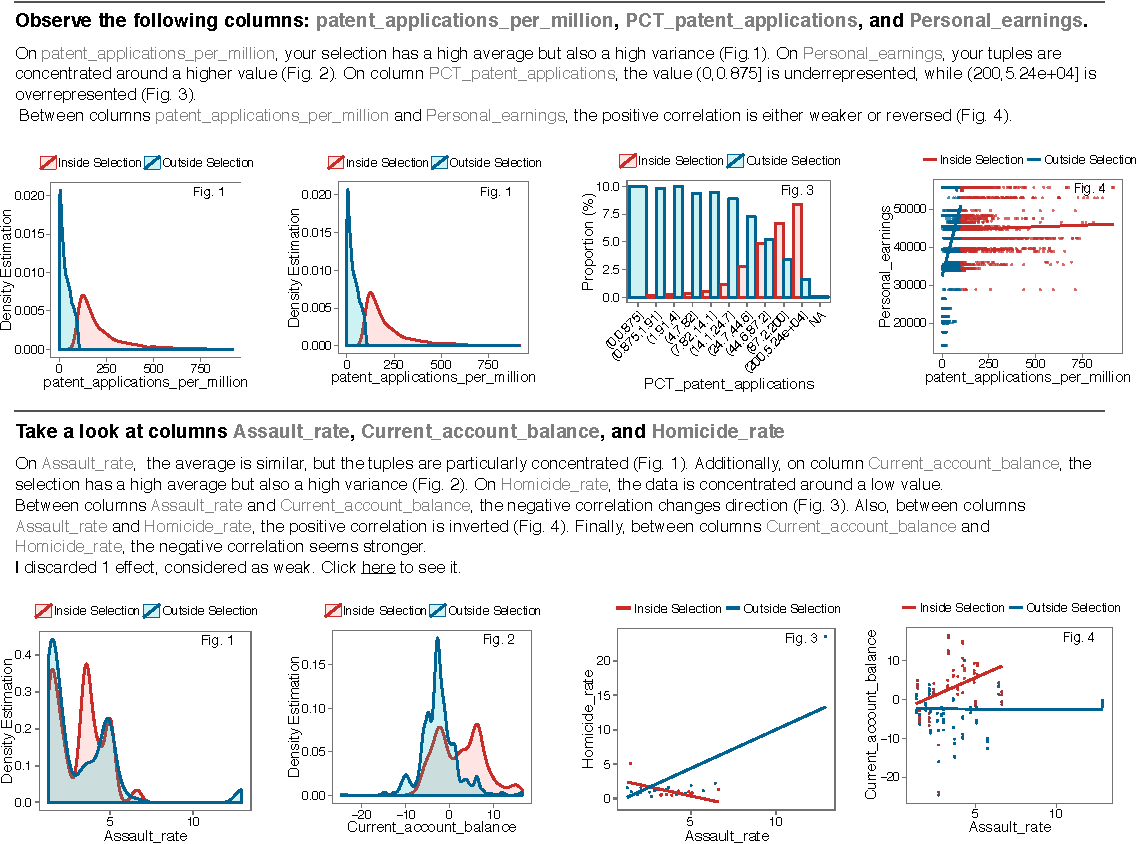
\includegraphics[width=2\columnwidth]{Figures/UseCase}
  \caption{Ziggy's explanations for Views 1 and 4}
  \label{pic:zigdetail}
\end{figure*}
We now apply Ziggy on the real use case which inspired our running example.
Our aim is to understand which factors lead to innovation, and more
specifically patents.  To answer this questions, we aggregated several
databases from the OECD, an international economic organization. All the data
we used may be found online\footnote{http://stats.oecd.org/}. Our core dataset
is the \texttt{Patents per Region} database, which contains 15 years of patent
statistics for 2,180 regions in 31 countries. We augmented this set with
several other region-level databases (\texttt{Demographics per Region} and
\texttt{Labour per Region}) and country-level indicators (\texttt{Better Life},
\texttt{Well Being} and \texttt{Innovation Indicators}).  We obtain a table
with about 6,823 rows and 519 columns, including mixed types and missing
values. We filtered out the categorical columns with more than 20 distinct
values (e.g., primary keys, countries and region names). 

Our selection of tuples contains the top 10\% regions for the statistic
\texttt{patent applications per million inhabitant}. We set $D=6$ with the
adaptive stopping method described in Section~\ref{sec:parameters}, and we used
$\mf{S}_{hard}$, with a maximum value of $L=0.75$.  Ziggy detects a total of 12
views, which columns are reported in Table~\ref{tab:ziggysviews}.

Some of Ziggy's choices were not surprising to us. For instance, the first
column mentioned in the Table is precisely the variable we used to define our
selection. The second one, $\texttt{PCT patent applications}$ is highly similar
(the PCT is an international patent treaty, which allows transnational
patents). Likewise, we expected some relationship between education and
innovation (views 2, 6 and 10). However, some effects are less straightforward.
How does \texttt{Employees working very long\- hours} impact innovation? Are
patents produced at work, or during hobby time? Similarly, how do our
innovative regions behave on the variable~\texttt{Job security}?

Figure~\ref{pic:zigdetail} presents Ziggy's explanations for two views. To
obtain this figure, we made only two edits: we removed some plots to save
space, and we inserted references to the charts in the text. Consequently, the
figure illustrates accurately what Ziggy's users would obtain. The first view
reflects the fact that innovative regions also have a high income. Ziggy
expresses this through its comments about the
variable~\texttt{Personal earnings}, but also through the last chart. As it
points out, there is a correlation between patent applications and income, but
this correlation disappears when we focus on innovative regions. Then, the
regression line is flat, with a high offset, which indicates that all these
regions are relatively rich, regardless of their patent statistics.

The second view offers a different perspective. The first and third charts show
that innovative regions tend to be safer, but the relationship is not
straightforward. Ziggy points out that these regions have less extreme values
on \texttt{Assault rate}, but the mean is similar. Also, the expected
correlation between \texttt{Assault rate} and \texttt{Homicide rate} is
inverted. This reflects the fact that assaults do exist in our innovative
regions, but little of them actually lead to a homicide. The last chart is more
puzzling: there normally exists no relationship between \texttt{Assault rate}
and \texttt{Current ac\-count balance}. And indeed, we expect these variables
to be independent, because they describe completely different topics. Yet,
in the innovative regions, a clear correlation appears. How can we interpret
this effect? If this dependence completely spurious? Alternatively, are those
variables cofounded by a third, hidden variable? Or maybe sane public accounts
causes anger among inventors? As implausible as this last hypothesis may seem, this
chart gives us no way to discard it. We leave the question open for future
investigations.

\section{Experiments}
\label{sec:experiments}



\textbf{Metrics.} We now present our experimental results. We want to evaluate
three aspects of our system: the \emph{quality} the views, their
\emph{diversity}, and Ziggy's \emph{runtime}. To evaluate the quality of the
views, we simulate users with statistical classifiers. We assume that if a
classifier can learn from a view, then so can a real user. Technically, we
materialize the user's selection into a vector $\rb{t} = (t_1, \ldots,
t_n)^\top$: $t_i=1$ if the tuple is chosen, 0 otherwise.  We then train a
classifier, using the view $\bf{D}^i$ as feature set and the user's selection
$\bf{t}$ as target. We then check if the classifier can accurately reconstruct
$\bf{t}$ from $\bf{D}^i$. If so, we deduce that the selection has a
recognizable structure in the subspace.  Therefore, the view contains
exploitable information. Oppositely, if the classifier cannot reconstruct the
user's selection, then either the classifier is poor, or the view contains no
information about the selection. We use a 5-Nearest Neighbor (5-NN) classifier,
and we report the F1 measure with 5 cross-validation (higher is better). We
chose the nearest neighbor algorithm for convenience: it is fast, and it gave
us good predictive performance. The
last two aspects are easier to quantify. To measure diversity, we report the
number of distinct columns used the set of views (higher is better). We measure
runtime with the total wall clock time - including preprocessing in Ziggy's
case (lower is better).

\textbf{Baselines.} We compare Ziggy to four state-of-the-art subspace
detection methods from the data mining literature. Our first three methods are
supervised: their aim is to detect informative sets of columns, in order to
predict a special, target column. We adapt these methods to our problem by
setting $\bf{t}$ as the target column. Here again, our rationale is the
following: if a set of column is a good predictor for the user's selection,
then it contains useful information.

Our first baseline is \texttt{Claude}, a recently published feature search
algorithm. We chose this method because it uses a multi-view approach, and
therefore its results are directly comparable to ours: like Ziggy, it returns a
fixed number of subspaces, with a user-specified number of dimensions.
Technically, Claude differs on two points. First, it uses a different notion of
interestingness: it seeks groups of columns which are strongly dependent to the
target, dependency being measured with the mutual information. Second, Claude
builds subspaces with a level-wise, beam search algorithm. We used the authors'
implementation.  We expect this approach to be both fast and accurate.

Our second baseline is \texttt{Clique}, inspired by the pattern mining
literature~\cite{xie2010max}. The idea is to build a graph inside which the
weight of each edge $(i,j)$ represents the statistical dependency between the
pair of columns $i,j$ and the target variable (again, we measure dependency
with the mutual information) . To obtain $K$ subspaces with at most $N$
variables, we remove all the edges except the $K' > K$ strongest, and detect
cliques of at most $N$ nodes in the remaining graph. By default, we set $K' =
2\cdot K$. To detect cliques, we used the \texttt{igraph} software package . We
expect this algorithm to be fast but rather approximative.

Our third baseline, \texttt{Wrap-5NN} is a ``wrapper'' from the feature
selection literature~\cite{guyon2003introduction}. This algorithm trains 5-NN
classifiers with increasingly large sets of variables. First, it tests each
variable, and it keeps the top $K$. Then, it tests combinations of two columns.
The process is repeated until the views reach $D$ dimensions. We chose 5-NN
because it is the algorithm we use to evaluate the views. We expect this
approach to be close to optimal, but also very slow. Thus, we only use it as a
``gold standard'' for our experiments with real data.

The last baseline, \texttt{4S}, detects subspaces in an unsupervised manner: it
seeks ``interesting'' subspaces, independently of the user's selection. More
precisely, it detects groups of variables which are strongly mutually
dependent, using an multivariate correlation measure. We used
the author's implementation written in Java. We expect $\texttt{4S}$ to be
fast, but also less accurate than its competitors because of it unsupervised
nature.

\textbf{Setup.} We implemented Ziggy in R, exploiting its native primitives for critical
operations (namely computing means, covariance matrices and cross-tabulation).
We interrupted all the experiments which lasted more than 1 hour. Our test
system is based on a 3.40 GHz Intel(R) Core(TM) i7-2600 processor. It is
equipped with 16 GB RAM, but the Java heap space is limited to 8 GB. All the
algorithms we present are single-threaded. The operating system is Fedora 16.

\begin{figure*}[t!]
  \centering
  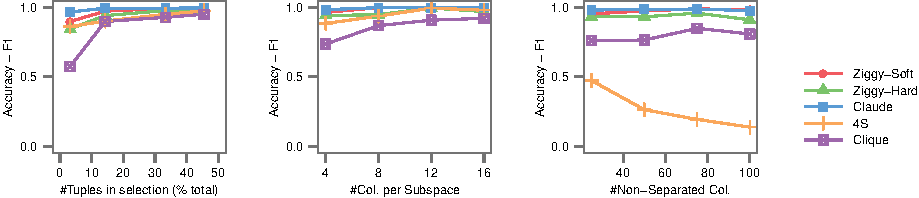
\includegraphics[width=\textwidth]{Plots/Synth-Accuracy}
  \caption{Average quality of the views varying the data generator parameters.}
  \label{pic:synthquali}
\end{figure*}
\begin{figure*}[t!]
    \centering
    \begin{subfigure}[b]{0.5\textwidth}
    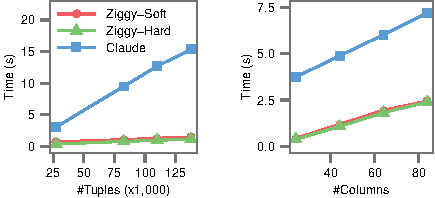
\includegraphics[height=4cm, width=\textwidth]{Plots/Synth-Runtime}
    \caption{Runtime for the three fastest algorithms, varying data parameters.
    The points for \texttt{Ziggy-Hard} and \texttt{Ziggy-Soft} overlap.}
    \label{pic:genruntime}
    \end{subfigure}
    ~~
    \begin{subfigure}[b]{0.45\textwidth}
        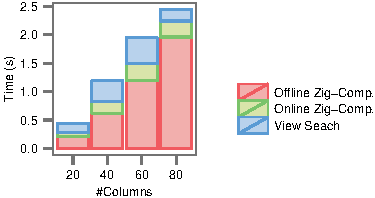
\includegraphics[height=4cm, width=\textwidth]{Plots/Synth-TimeDetail}
        \caption{Breakdown of the total runtime for \texttt{Ziggy-Soft},
        varying the number of columns.}
    \label{pic:detruntime}
    \end{subfigure}
  \label{pic:syntruntime}
    \caption{Runtime experiments with synthetic data.}
\end{figure*}
\begin{figure}[t!]
  \centering
  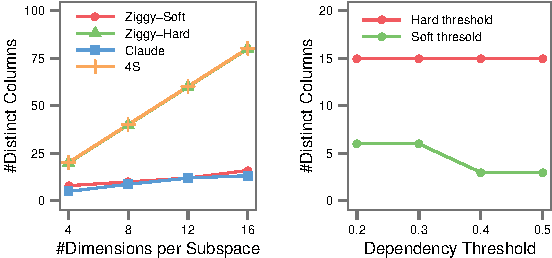
\includegraphics[width=\columnwidth]{Plots/Synth-Dedup}
  \caption{Variety of the views.}
  \label{pic:synthvariety}
\end{figure}
\begin{table}[t!]
    \centering
    \small
    \begin{tabularx}{\columnwidth}{X  c }
      \hline
      Parameter & Value\\
      \hline
      Selection (tuples) & 3,000\\
      Tuples from Gauss. mixture & 15,000\\ 
      Tuples from Unif. distrib. & 15,000\\
      Sep. / Non-sep. variables & 20 / 4\\
      \hline
      Num. dimensions subspaces & 4\\
      Num. components Gaussians& 5\\
      Mean / Variance Gaussians & Unif. in [-10,10] / [1, 20]\\
      Uniform noise & Unif. in [-45,45]\\
      \hline
    \end{tabularx}
    \caption{Default parameters for our data generator.} 
\label{tab:synthparameters}
\end{table}

\subsection{Synthetic Data}
\label{sec:synthexp}


In this set of experiments, we benchmark our algorithms in a synthetic
environment. Since we know the structure of the data in advance, we can tune
the competitors optimally. For instance, if we generate a dataset with 3
subspaces of 5 columns, then we set $K=3$ and $D=5$. We must however report
that \texttt{4S} tunes itself: it computes how many subspaces to generate, and
how large these should be. We use two versions of Ziggy: for
\texttt{Ziggy-Soft} we use the dependency measure $\mf{S}_{soft}$ and we limit
it to 0.1. For \texttt{Ziggy-Hard}, we use $\mf{S}_{hard}$ and we limit it
to~0.9.

Our generator produces columns by groups. It
yields two types of subspace: \emph{non-separated} subspaces, and
\emph{separated} subspaces. In the non-separated case, the selection and the
rest of the data are sampled from the same distribution, namely a mixture of
multivariate Gaussians with random parameters. In the separated case, the
selection is sampled from a separate Gaussian distribution, with its own random
parameters. Additionally, our generator produces uniform noise on all the
columns. Table~\ref{tab:synthparameters} presents our parameters. For each
experiment, we generate 4 random data sets and report the average F1 of all the
views.

\textbf{Quality of the Views.} The first chart in Figure~\ref{pic:synthquali}
presents the robustness of the algorithms with regards to the size of the
selection. For all our baselines, raising this parameter ameliorates the views, 
but the quality converges fast (at around 15\% of the database size).  The
algorithm \texttt{Claude} comes first, but it is very closely followed by the
two instances of \texttt{Ziggy} and \texttt{4S}. The ranking is almost
identical in the second chart, which displays the accuracy of the algorithms
varying the dimensionality of the subspaces. All algorithms involved seem
robust, but \texttt{Ziggy-Soft}, \texttt{Ziggy-Hard} and \texttt{Claude}
are above, followed closely by \texttt{4S}, then
\texttt{Clique}. The last graph illustrates the robustness of the views with
regards to the number of non-separated columns.  All our baselines achieve good
scores, except \texttt{4S}. We interpret this effect by the fact that
\texttt{4S} is unsupervised, it has therefore now way to detect which subspaces
are interesting and which are not. In conclusion, despite its simple
assumptions, Ziggy delivers high quality, robust views, largely comparable to
state-of-the-art feature selection algorithms.

\textbf{Runtime.} Figure~\ref{pic:genruntime} illustrates the total runtime
with regards to the number of rows and columns in the database. We ignored the
algorithms \texttt{4S} and \texttt{Clique}, which were slower than the
other candidates. We observe that Ziggy's performance is spectacular: it is
an order of magnitude faster than \texttt{Claude}, which is itself faster than
the other competitors. And yet, all the algorithms involved in our benchmark
have the same $\mathcal{O}(ND^2)$ complexity. We explain the difference with Ziggy's
simpler computations, which reduce the constant factor. For instance, Claude
needs to estimate the mutual information between possible pair of columns and
$\bf{t}$. In comparison Ziggy compares every pairs of correlations inside
and outside the selection. This operation has the same complexity, but is is
much faster since it involves no binning, logarithms or branching - it involves
little more than scans.

Figure~\ref{pic:detruntime} shows where \texttt{Ziggy-Soft} spends its time.
By far, the most expensive operations are the offline computations. This
validates our staging strategy.  Table~\ref{tab:synthparameters} reports that
the database contains 1 selected tuple for every 10 non selected tuple.
Therefore we expected the online phase to be about 10 times faster, ignoring
overhead costs. The figure confirms this estimation.

\textbf{Diversity.} Figure~\ref{pic:synthvariety} presents the number of
distinct co\-lumns mentioned in the views. In the leftmost
chart, we compare four competitors, varying the width of the subspaces. We
notice two distinct groups of columns. The approaches \texttt{Ziggy-Hard} and
\texttt{4S} offer a very high diversity, because they enforce that no columns
is shared among subspaces. The approaches \texttt{Claude} and
\texttt{Ziggy-Soft} offer much less variety. The rightmost figure illustrates
the effect of the dependency threshold. In the Hard case, it has no apparent
effect because the views are completely disjoint anyway (the threshold  does
separate the correlated columns, but this does not influence our metric). In
the Soft case, we see that a lower threshold forces Ziggy to introduce variety.


\subsection{Real Data}
\label{sec:realdata}

\begin{figure*}[!ht]
  \centering
  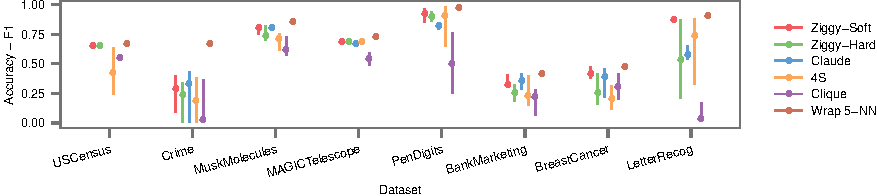
\includegraphics[width=0.8\textwidth]{Plots/Real-Accuracy}
  \caption{Quality of the views. The points represent median scores, the bars
  represent the lowest and greatest scores.}
  \label{pic:realquali}
\end{figure*}
\begin{figure*}[!ht]
  \centering
  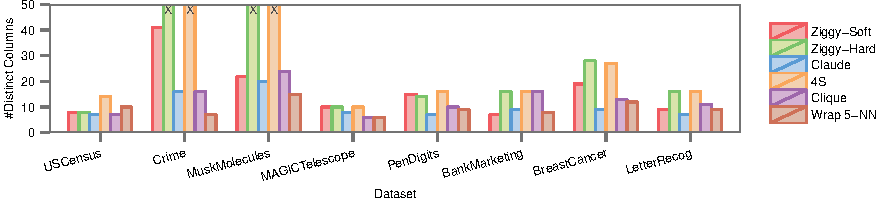
\includegraphics[width=0.8\textwidth]{Plots/Real-Diversity}
  \caption{Diversity of the views. The \texttt{X} mark indicates that we 
  truncated the column.}
  \label{pic:realdiversity}
\end{figure*}
\begin{figure*}[!ht]
  \centering
  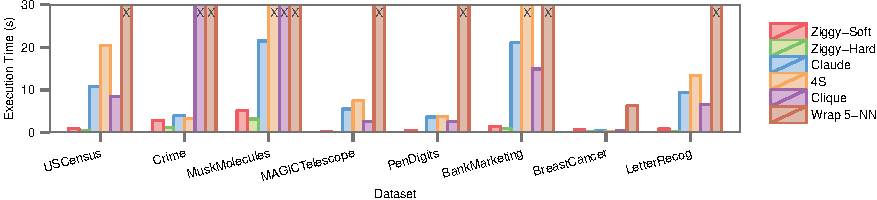
\includegraphics[width=0.8\textwidth]{Plots/Real-Runtime}
  \caption{Runtime. The \texttt{X} mark indicates that we truncated the column.}
  \label{pic:realruntime}
\end{figure*}
We now presents our experiments on real data from the UCI Repository. We
introduce the algorithm \texttt{Wrap-5NN}, which we use as ``gold standard'',
since it optimizes precisely the metric we report. To set the parameters, we
rely on \texttt{4S}. Recall that this algorithm has a built-in mechanism to
pick the best values. Thus, we run it first, then we count how many views it
generated and how large these views are (if the number of columns is not
constant, we take the average). We then apply these setting to all the other
algorithms. Table~\ref{tab:datasets} describes the datasets. Because all the
competitors have the same parameters, the comparison is fair.

\textbf{Accuracy.} Figure~\ref{pic:realquali} illustrates the quality of the
views for each algorithm. We observe that \texttt{Wrap 5-NN} comes always
first. It is followed by \texttt{Claude}, \texttt{Ziggy-Soft} and
\texttt{Ziggy-Hard}, often closely (although \texttt{Crime} is a striking
counter-example) and in different orders. The unsupervised
\texttt{4S} follows in most cases, tailed by \texttt{Clique}. Here again, we
conclude that Ziggy's performance is largely comparable to good feature
selection algorithms. However, we observe that \texttt{Ziggy-Hard} is often
below \texttt{Ziggy-Soft}, the most extreme case being the \texttt{LetterRecog}
set.  This is a consequence of its diversity. In the synthetic case, Ziggy had
several equally good subspaces to chose from. In the last three datasets, it
seems that some subspaces are better than others, and therefore non-redundancy
induces an accuracy loss (observe that \texttt{4S} suffers from the same
problem).

\textbf{Diversity.} Figure~\ref{pic:realdiversity} presents the diversity results.
As with synthetic data, we observe that \texttt{4S} and \texttt{Ziggy-Hard}
dominate the other algorithms, in particular with wide datasets such as
\texttt{Crime} and \texttt{MuskMolecules}. The algorithms \texttt{Ziggy-Soft}
and \texttt{Clique} follow, and \texttt{Wrap-5NN} comes last - which we
expected since \texttt{Wrap-5NN} targets accuracy only. This chart, in
conjunction with Figure~\ref{pic:realquali}, shows that the algorithms which
generate the best F1 rarely generate the best diversity, and reciprocally. This
motivates our choice to offer both $\mf{S}_{Hard}$ and $\mf{S}_{Soft}$.

\textbf{Runtime} We present the runtime of our algorithms in
Figure~\ref{pic:realruntime}. The results are consistent with our previous
conclusions: Ziggy outperforms all of its competitors, and the speedup gets more
dramatic as the size of the datasets increase.


\section{Related Work}
\label{sec:related-works}
\begin{table}[!t]
    \centering
    \small
    \begin{tabular}{r c c c c} 
        \hline
        Dataset & Columns & Rows & \#Views & Dim Views\\
        \hline
        MuskMolecules & 167 & 6,600 & 22 & 18\\
        Crime & 128 & 1,996 & 20 & 17\\
        BreastCancer & 34 & 234 & 10 & 13\\
        PenDigits & 17 & 7,496 & 9 & 10\\
        BankMarketing & 17 & 45,213 & 11& 8\\
        LetterRecog & 16 & 20,000 & 10 & 12\\
        USCensus & 14 & 32,578 & 10 & 7\\
        MAGICTelescope & 11 & 19,022 & 1 & 10\\
        \hline
    \end{tabular}
    \caption{Characteristics of the datasets. The last two columns are used for
    comparison with 4S.}
    \label{tab:datasets}
\end{table}

{\color{red} TO DO}

\textbf{Feature Selection.} Feature selection seeks columns of $\rb{V}$ from
which we can predict $\rb{t}$. Ultimately, the goal is to estimate
$p(t|\rb{x})$. Our problem is symmetric: we seek columns of $\rb{V}$ which are
influenced by $\rb{t}$. Hence, we focus on $p(\rb{x}|t)$. According to Bayes'
theorem, these two problems are equivalent. And indeed, some feature selection
methods, such as LDA, are also based on $p(\rb{x}|t)$. But the differences do
not stop here.  Recall we focus on interpretation, while feature selection
algorithms target prediction. Therefore, we seek a few, non-redundant views,
while classic algorithms focus on single, potentially complex views. Also, most
feature selection algorithms optimize class separability. In this paper, we are
interested in any kind of dissimilarity. For instance, most feature selection
algorithms would reject the view presented in Figure~\ref{pic:sameMean}. For
us, this view is perfectly acceptable. 

{\color{red} Big TODO: contrast with Bailey's approach.
I still have to read about metric learning.}


\section{Conclusion}
\label{sec:conclusions}




%\section*{[Private] Appendix: Ziggy vs.Claude}
%\label{zigvsclaude}
%We may now wonder: if we set $\mf{D}$ as the KL divergence, what is the
%difference between Claude and Ziggy?  Suppose that we ignore the penalty factor
%(we set $\lambda=0$). Then Ziggy tries to maximize:
%$$
%KL\big(\rb{x} | t=0 \ ; \  \rb{x} | t=1 \big)
%$$
%Intuitively, this is the distance between $\rb{x} | t=0$ and $\rb{x} | t=1$.
%On the other hand, Claude maximizes $I(\rb{x}, t)$. With a bit of playinFirst, look at columns AvgIncome and YearsOfEducation. Observe that the mean….g
%around, we can show that this is equivalent to maximizing:
%$$
%    KL\big(\rb{x} | t=0 \ ; \  \rb{x} \big) + 
%        KL\big(\rb{x} | t=1 \ ; \  \rb{x} \big)
%$$
%Here, we are interested in the distance between $\rb{x} | t=i$ and a central
%distribution $\rb{x}$. 
%
%There is a triangular relationship between these expressions:
%\begin{figure}[h!]
%  \centering
%  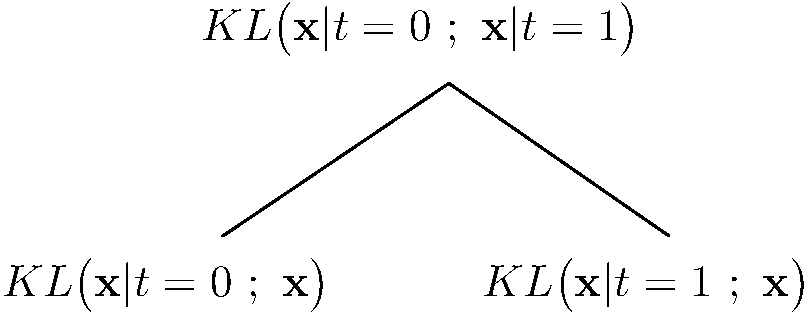
\includegraphics[width=0.6\columnwidth]{Figures/Triangle}
%  \label{pic:triangle}
%\end{figure}
%
%I wonder if they are not actually equivalent!


